\section{Milestone II}\label{sec:m2}

The main goal of this section is to investigate the recombination history of the universe. This can be explained as the point in time when photons decouple from the equilibrium of the opaque, early universe.  When this happens, photons scatter for the last time at the \textit{time of last scattering}, and these photons are what we today observe as the CMB. This period of the history of the universe is thus crucial for understanding the CMB. 

We will start by calculating the free \textit{electron fraction} $X_e$, from which we may find the \textit{optical depth} $\tau$. This again enables us to compute the \textit{visibility function}, $g$, and the \textit{sound horizon}, $s$. The latter will be of great importance later. 

Recombination happens because the expansion of the Universe cools it down, making the photons less energetic, which in turn make each interaction in the primordial plasma less energetic. At some point, hydrogen atoms are able to form, reducing the number of free electron, hence reducing photon interactions, until they scatter for the last time. We will determine the time of recombination from the free electron fraction, which indirectly tell us how large portion of the free electron have (re)-combined.\footnote{As with any good article on the subject, we ought to say that recombination is a funny wording, as this is the first time in the history of the Universe that protons and electrons combine to form hydrogen.} Due to the decrease of free electron, photons interact less with them (optical depth is decreased). At some point, photons scatter for the last time, and this information is encapsulated in the visibility function. 


\subsection{Theory}\label{sec:m2:theory}
    In order to explain the inventory of the universe, we need to understand how the distribution of different species changes over time. This is governed by the \textit{Boltzmann equation},
    \begin{equation}\label{eq:m2:theory:bolzmann_def}
        \dv{f}{t} = C[f],
    \end{equation}
    where $f(\vec{x},\vec{p},t)$\footnote{Given in \textit{phase-space coordinates}: ($x^\mu,P^\mu$)} is the distribution function of a given species. $C[f]$ are the collision terms, which depends on the species through the same distribution function $f$. Due to the function dependencies of $f$ we are able to generally expand it into ~\cite[Eq. 3.33]{dodelson2020modern}:
    \begin{equation}\label{eq:m2:theory:bolzmann_expanded}
        \dv{f}{t} = \pdv{f}{t}+\pdv{f}{x^i}\dv{x^i}{t} + \pdv{f}{p}\dv{p}{t} + \pdv{f}{\hat{p}^i}\dv{\hat{p}^i}{t} = C[f],
    \end{equation}
    where $p=\abs{\vec{p}}$ and $\hat{p}=\vec{p}/p$.

    Before recombination, the equilibrium between protons, electrons and photons is governed by the following interaction, from ~\cite{weinberg2008cosmology}\footnote{Where $H^*$ denotes excited states of hydrogen which will decay into neutral hydrogen.}:
    \begin{equation}\label{eq:m2:theory:equilibrium_interaction}
        e^-+p^+\leftrightharpoons H^* + \gamma,
    \end{equation}
    where a proton and an electron interact to form an excited hydrogen atom, which decays and emits a photon, or a photon excites and split a hydrogen atom into a free electron and a proton through \textit{Compton scattering}.\footnote{Elastic scattering of photons is technically Thomson scattering, but Compton scattering is a more general term and will be used (~\cite{dodelson2020modern}). This is also why we later use the Thomson cross section $\sigma_T$. The reaction is when a photon scatters of an electron, and possibly energises it enough to break out of the hydrogen atom, if already bound: $$\gamma + e^- \leftrightharpoons \gamma+e^-.$$} ~\cref{eq:m2:theory:equilibrium_interaction} is a reaction of the form $1+2\leftrightharpoons 3+4$, and we have from ~\cite{AST5220LectureNotes} that the Boltzmann equation for such a reaction is:
    \begin{equation}\label{eq:m2:theory:boltzmann_eq}
        \frac{1}{n_1e^{3x}}\dv{(n_1e^{3x})}{x} = -\frac{\Gamma}{H}\left(1-\frac{n_3n_4}{n_1n_2}\left(\frac{n_1n_2}{n_3n_4}\right)_\mathrm{eq}\right),
    \end{equation}
    where $n_i$ are the number densities of the reactants, $\Gamma$ is the reaction rate and $H$ the Hubble parameter (expansion rate of the universe). If the reaction rate is much larger than the expansion rate of the universe, $\Gamma \gg H$, then ~\cref{eq:m2:theory:equilibrium_interaction} ensures equilibrium between protons, electron and photons. When $\Gamma$ drops below $H$, then the expansion rate becomes dominant and the reaction rate is unable to sustain equilibrium. This happens when the temperature of the Universe becomes lower than the binding energy of hydrogen, hence stable neutral hydrogen is able to form.\footnote{Well, it is really not as simple, as neutral hydrogen is obtained from excited hydrogen and how this process go about is non-trivial. As we ignore re-ionisation, I will not delve into this. However, both ~\cite[p. 113-129]{weinberg2008cosmology}, ~\cite[p. 95-99]{dodelson2020modern} and ~\cite{AST5220LectureNotes} elaborate further on this.} As a consequence, the photons \textit{decouple} from the protons and electron. When $\Gamma \ll H$, there are practically no interactions and the number density becomes constant for a comoving volume. Massive particles \textit{freeze out} and their abundance become constant. 

\subsubsection{Hydrogen recombination}\label{sec:m2:theory:hydrogen_recombination}
    We express the electron density through the free electron fraction $X_e \equiv n_e/n_\mathrm{H} = n_e/n_b$ where we have assumed that hydrogen make up all the baryons ($n_b=n_\mathrm{H}$). We also ignore the difference between free protons and neutral hydrogen. From ~\cite{https://doi.org/10.48550/arxiv.astro-ph/0606683} we obtain:
    \begin{equation}\label{eq:m2:theory:baryon_number_density}
        n_b = \frac{\rho_b}{m_\mathrm{H}} = \frac{\O_b\rho_c}{m_\mathrm{H}}\expe{-3x},
    \end{equation}
    where $m_\mathrm{H}$ is the mass of the hydrogen atom, and $\rho_c$ the critical density today as defined earlier. Before recombination, no stable neutral hydrogen is formed, thus the electron and baryon density is the same, i.e. there are only free electrons so $X_e \simeq 1$. When in equilibrium, the r.h.s. of ~\cref{eq:m2:theory:boltzmann_eq} reduces to 0, which is called the \textit{Saha approximation}. The solution is in this regime described by the \textit{Saha equation}, which from ~\cite{dodelson2020modern} in physical units is:
    \begin{equation}\label{eq:m2:theory:Saha_equation}
        \frac{X_e^2}{1-X_e} = \frac{1}{n_b}\left(\frac{k_Bm_eT_b}{2\pi\hbar^2}\right)^{3/2}\expe{-\epsilon_0/k_BT_b},
    \end{equation}
    where $\epsilon_0 = 13.6\text{ eV}$ is the ionisation energy of hydrogen. The Saha equation is only a good approximation when $X_e \simeq 1$. Thus for $X_e < (1-\xi)$,\footnote{Where $\xi$ is some small tolerance, which have to be defined in some numerical model for when to abonden the Saha equation and use the more accurate, but computationally more expensive Peebles equation. This is typically $\xi=0.001$} which corresponds to the period during and after recombination, we have to make use of the more accurate \textit{Peebles equation}. From ~\cite{https://doi.org/10.48550/arxiv.astro-ph/0606683}:
    \begin{subequations}\label{eq:m2:theory:peebles_equation}
        \begin{equation}
            \dv{X_e}{x} = \frac{C_r(T_b)}{H}\left[\beta(T_b)(1-X_e)-n_\mathrm{H}\alpha^{(2)}(T_b)X_e^2\right],
            \tag{\ref{eq:m2:theory:peebles_equation}}
        \end{equation}
        where
        \begin{align}
                C_r(T_b) &= \frac{\Lambda_{2s-1s}+\Lambda_\alpha}{\Lambda_{2s-1s} + \Lambda_\alpha+\beta^{(2)}(T_b)},\label{eq:m2:theory:peebles_CR} \\
                \Lambda_{2s-1s} &= 8.227 \unit{s}^{-1}, \label{eq:m2:theory:peebles_lambda}\\
                \Lambda_\alpha &= \frac{1}{(\hbar c)^3}H\frac{(3\epsilon_0)^3}{(8\pi)^2n_{1s}}, \label{eq:m2:theory:peebles_lambda_alpha}\\
                n_{1s} &=(1-X_e)n_\mathrm{H}, \label{eq:m2:theory:peebles_ns}\\
                n_\mathrm{H} &= (1-Y_p)\frac{3H_0^2\O_{b0}}{8\pi Gm_\mathrm{H}}\expe{-3x}, \label{eq:m2:theory:peebles_nH}\\
                \beta^{(2)}(T_b) &= \beta(T_b)\expe{3\epsilon_0/4k_BT_b}, \label{eq:m2:theory:peebles_beta2}\\
                \beta(T_b) &= \alpha^{(2)}(T_b)\left(\frac{k_Bm_eT_b}{2\pi\hbar^2}\right)^{3/2}\expe{-\epsilon_0/k_BT_b}, \label{eq:m2:theory:peebles_beta}\\
                \alpha^{(2)}(T_b) &=\frac{\hbar^2}{c}\frac{64\pi}{\sqrt{27\pi}}\frac{\alpha^2}{m_e^2}\sqrt{\frac{\epsilon_0}{k_BT_b}}\phi_2(T_b), \label{eq:m2:theory:peebles_alpha}\\
                \phi_2(T_b) &= 0.448\ln\left(\frac{\epsilon_0}{k_BT_b}\right). \label{eq:m2:theory:peebles_phi2}
        \end{align}
    \end{subequations}

    The Peebles equation takes into account that the energy (excitation) of hydrogen formed through ~\cref{eq:m2:theory:equilibrium_interaction} vary, and that decays take place until we reach the $n=2$ level (first excited state), denoted by $^{(2)}$ in ~\cref{eq:m2:theory:peebles_CR}-~\cref{eq:m2:theory:peebles_phi2}. Recombination to the ground state is not relevant, as this leads to an ionised photon which immediately ionises a neutral hydrogen atom ~\cite[p. 97]{dodelson2020modern}. The $C_r$ is the probability that singly ionised hydrogen is reionised further, where $\beta^{(2)}$ and $\beta$ are the collisional ionisations from the first ionised state and ground state respectively. $\alpha^{(2)}$ is the recombination rate to excited states. For more detailed description of these terms, see ~\cite{Ma_1995}. \footnote{Because of this non-trivial path into the ground state, and the large photon to baryon number ratio, recombination happens later than when the temperature of the universe correspond to exactly the binding energy of neutral hydrogen (~\cite{https://doi.org/10.48550/arxiv.astro-ph/0606683})}

    We find $X_e$ by solving ~\cref{eq:m2:theory:Saha_equation} for $X_e > (1-\xi)$ and ~\cref{eq:m2:theory:peebles_equation} for $X_e < (1-\xi)$. In theory, it is possible to solve the Peebles equation at very early times, but the equation is very stiff resulting in unstable numerical solutions at early times (high temperatures), hence the Saha approximation.

\subsubsection{Visibility}\label{sec:m2:theory:visibility}
    Visibility is a concept tied to the optical depth and mean free path of a medium. The two latter are inversely proportional to each other. The mean free path is the average distance a photon travels before its direction is changed (often by scattering). Thus, a small mean free path gives results in a lot of collision across short distances, which occurs in optically thick media. The optical depth as a function of conformal time is defined as \cite{AST5220LectureNotes}:
    \begin{equation}\label{eq:m2:theory:optical_depth}
        \tau = \int_\eta^{\eta_0} n_e\sigma_\mathrm{T}\expe{-x}\d\eta',
    \end{equation}
    where $n_e$ is the electron density and $\sigma_\mathrm{T}$ is the Thompson cross-section. In differential form, restoring original units, this is:
    \begin{equation}\label{eq:m2:theory:optical_depth_differential}
        \dv{\tau}{x} = -\frac{cn_e\sigma_Te^x}{\Hp}.    
    \end{equation} 
    From this we define the visibility function, $g$:
    \begin{equation}\label{eq:m2:theory:visibility_function}
        \begin{split}
            g &= -\dv{\tau}{\eta}\expe{-\tau} = -\Hp\dv{\tau}{x}\expe{-\tau}\\
            \tilde{g} &\equiv -\dv{\tau}{x}\expe{-\tau} = \frac{g}{\Hp},
        \end{split}
    \end{equation}
    where $\tilde{g}$ is in terms of the preferred time variable, $x$. Notable thing about the visibility function $\tilde{g}$ is that it is a true probability distribution, describing the probability density of some photon to last have scattered at time $x$. Because of this, we have that $\int_{-\infty}^0\tilde{g}(x)\d x = 1$. We also take note of the derivative of the visibility function:
    \begin{equation}\label{eq:m2:theory:visibility_function_deriv}
        \dv{\tilde{g}}{x} = e^{-\tau}\left[\left(\dv{\tau}{x}\right)^2-\dv[2]{\tau}{x}\right]
    \end{equation}


\subsubsection{Sound horizon}
    Let's take a small step back and consider the situation of the early Universe. Before any decoupling, the photons and electrons are coupled through Thompson scattering, and protons and electrons are coupled through coulomb interactions. Because of this, photons interact with baryons and move alongside with them as one fluid, in which wave propagates with a speed $c_s$, from ~\cite{dodelson2020modern}:
    \begin{equation}\label{eq:m2:theory:sound_speed}
        c_s \equiv c\left[3(1+R)\right]^{-\frac{1}{2}} \quad ; \quad R\equiv\frac{3\O_b}{4\O_\gamma},
    \end{equation}
    where $R$ is the \textit{baryon-to-photon energy ratio}. By the definition of $R$, if the baryon density is negligible compared to the radiation density, $R\sim0$, and we recover the wave propagation speed in a relativistic fluid: $c_s=3^{-1/2}$ (~\cite{dodelson2020modern}). The total distance such a wave would have travelled in a time $t$ (since the beginning of the Universe) is called the \textit{sound horizon}, found by simply integrating $c_s$ through time, accounting for the expansion of space itself by including a factor $e^{-x}$:
    \begin{equation}\label{eq:m2:theory:sound_horizon_def}
        s = \int_0^tc_se^{-x}\d t = \int_{-\infty}^x\frac{c_s}{\Hp}\d x,
    \end{equation}
    where the variables are changed to $x$. On differential form:
    \begin{equation}\label{eq:m2:theory:sound_horizon_differential}
        \dv{s}{x} = \frac{c_s}{\Hp},
    \end{equation}
    which is a straightforward differential equation to solve given some initial conditions. 
\subsection{Methods}\label{sec:m2:methods}

some methods
\subsection{Results and discussion}\label{sec:m2:results} 

    \subsubsection{Times and sound horizon}
    The relevant times for last scattering, recombination and Saha recombination are obtained as explained in ~\cref{sec:m2:methods:analysis}, and presented in ~\cref{tab:m2:recomb_analysis}. These times are given in terms of $x$, the redshift $z$ and the cosmic time $t$ (in Myr). The sound horizon is given in units of megaparsecs (Mpc). Last scattering occurred when $x=-6.9853$, at redshift $z=1079.67$, which is slightly after recombination when $x=-6.9855$ at redshift $z=1079.83$. If the Saha approximation was valid when the electron fraction dropped, recombination would have happened when $x=-7.1404$ at redshift $1260.89$ which is significantly earlier. However, this is not the case since photons drop out of equilibrium with the primordial plasma as soon as hydrogen begin to form, and the free electron fraction is reduced. Thus, this number may only be used for comparison. Another thing worth noting is the validity of these numbers.
    \begin{table}
        \label{tab:m2:recomb_analysis}
        \begin{tabular}{l|rrrr}
\hline
Phenomenon & $x$ & $z$ & $t$ [Myr] & $r_s$ [Gyr] \\
\hline
Last scattering   & -6.99 & 1082.29 & 0.377 & 55394.8 \\
Recombination     & -6.99 & 1079.83 & 0.378 & 55590.6 \\
Saha              & -7.14 & 1260.89 & 0.291 & 43620.6 \\
\hline
\hline
\end{tabular}

        \caption{The times of last scattering and recombination given in terms of $x$, the redshift $z$, the cosmic time $t$ and the sound horizon $r_s$. Also included is the time of recombination found using the Saha approximation only.}
    \end{table}

    \subsubsection{Free electron fraction}
    ~\cref{fig:m2:electron_fraction} shows the free electron fraction $X_e$ as a function of $x$ found using both the Saha and Peebles equation, as explained in ~\cref{sec:m2:methods:electron_fraction}, in blue. Also shown is the results found from the Saha equation only, which tends to zero a lot faster. This is used for comparison only, as we have already stated that the Saha approximation is only valid for $X_e\simeq 1$. The time of recombination is shown for both cases, which for the Saha approximation happens significantly earlier than what is the actual case. The Peebles solution falls off gradually, and converges towards a constant value, which is the present day abundance of free electrons (freeze out abundance). This is found to be $X_e(x=0) = 0.0002$, shown as a brown dashed line in ~\cref{fig:m2:electron_fraction}.

    Since the Peebles equation is a solution of the Boltzmann equation, it takes into account the particle interaction with changing abundance, after the photons decouple from the primordial plasma. It is thus expected that this will result in a much more gradual fall off of the free electron fraction, just as we observe in ~\cref{fig:m2:electron_fraction}.
    \begin{figure}
        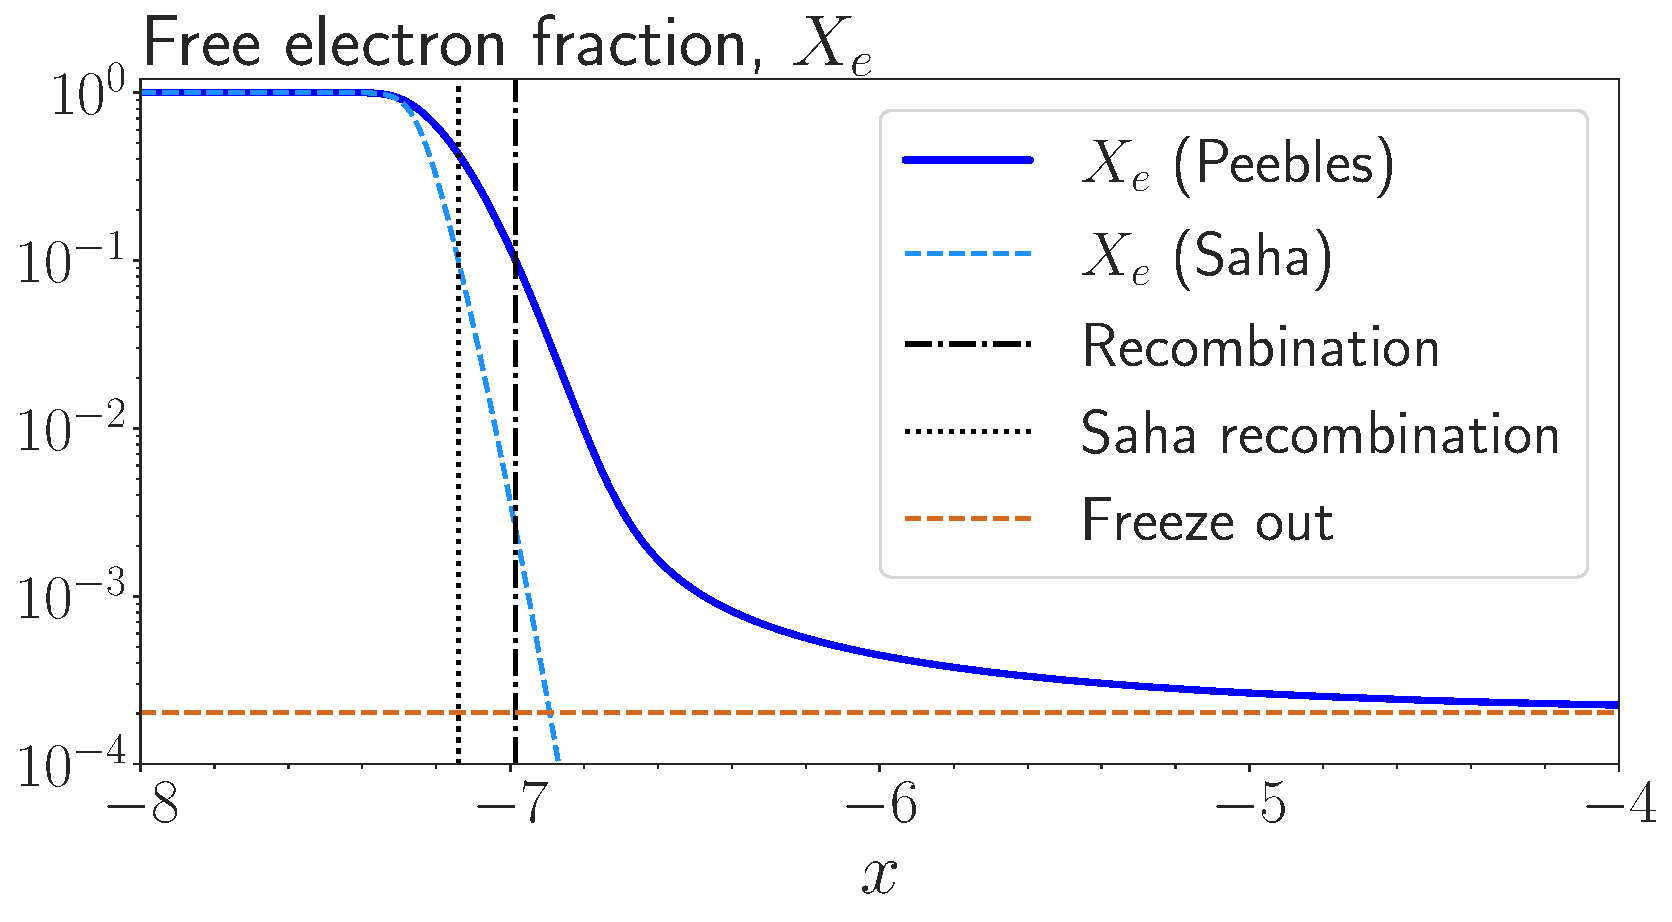
\includegraphics[width=\linewidth]{Xe_plot.pdf}
        \caption{The free electron fraction $X_e$ as function of $x$, found from the Saha and Peebles equation (blue). The result using only the Saha equation is shown in dashed light blue. The time of recombination is shown as a dashed black line. Likewise, recombination in the Saha approximation is shown as a dotted black line, appearing earlier. The freeze out abundance of hydrogen (the present value) is shown as a brown dashed line.}
        \label{fig:m2:electron_fraction}
    \end{figure}

    \subsubsection{Visibility}

    ~\cref{fig:m2:optical_depth} shows the optical depth and its first two derivatives as functions of $x$. This is a function of the time $x$, and thus the optical depth at some value is the integral of ~\cref{eq:m2:theory:optical_depth} from that time until today; it is cumulative. The surface of last scattering is shown with a black dashed line, before which the primordial plasma is optically thick, meaning the photons have a short mean free path. The decrease of the optical depth means that the photons gradually travel longer distances before interacting with free electrons. There are two processes going on here; the expansion of space itself, and the formation of neutral hydrogen. Both of which contribute to the increased mean free path of the photons. The contribution from the expansion of space is slow compared to the seemingly rapid change in the free electron fraction once neutral hydrogen is able to form. Thus, the rapid decrease of free electrons, as seen is ~\cref{fig:m2:electron_fraction} makes the mean free paths of photon to increase beyond the horizon. This effectively enable them to travel through space without interacting with matter, and this is what we observe as the CMB today - the Universe becomes transparent. This sudden decrease of optical depth is clearly seen in ~\cref{fig:m2:optical_depth}, both in $\tau$ itself, but also in its derivatives.
    \begin{figure}
        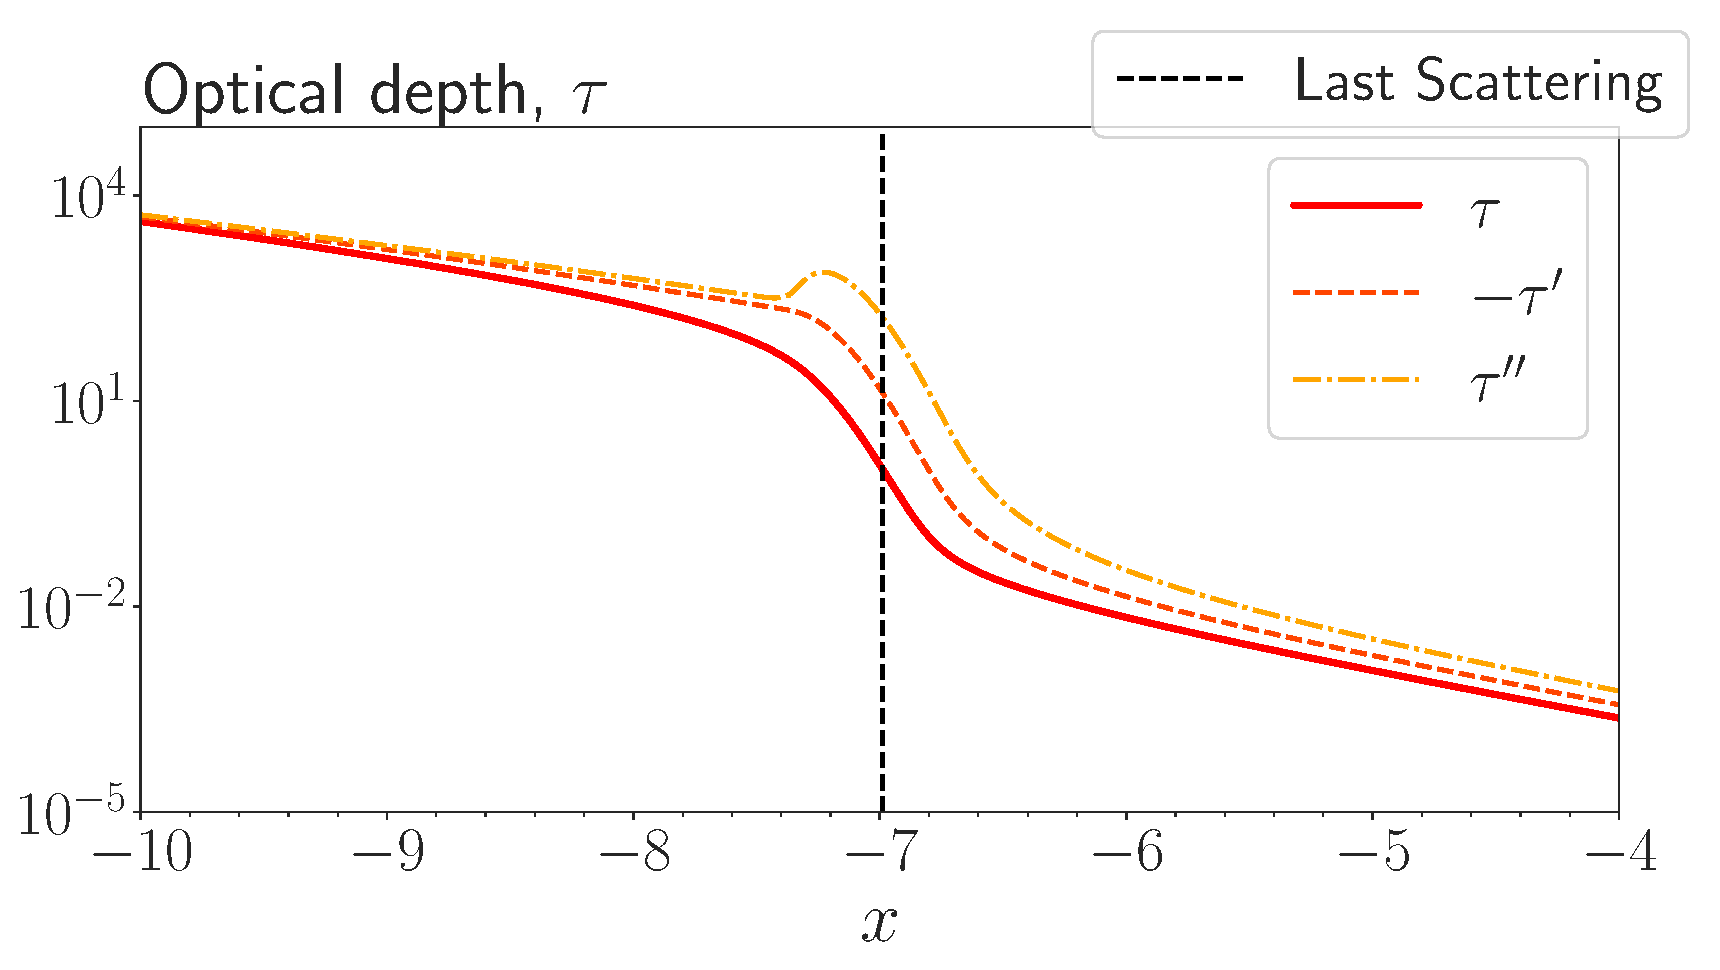
\includegraphics[width=\linewidth]{optical_depth.pdf}
        \caption{The optical depth $\tau$ and its first and second derivatives as functions of $x$. The time of last scattering is shown as a dashed black line, before which the Universe was optically thick.}
        \label{fig:m2:optical_depth}
    \end{figure}

    Another way of arriving at similar conclusions is by considering the visibility function in ~\cref{fig:m2:visibility_function}. Here, $\tilde{g}$ is shown in green along with its derivatives. The scaling follow that of ~\cite{https://doi.org/10.48550/arxiv.astro-ph/0606683}, in order to fit the graphs into the same figure. $\tilde{g}$ describes the probability that a photon reaching us today scattered at time $x$. The peak of this function indicates the time were \textit{the most} photons scattered for the last time, and is thus used as a definition of the last scattering surface. The visibility function is skewed forward in time.
    \begin{figure}
        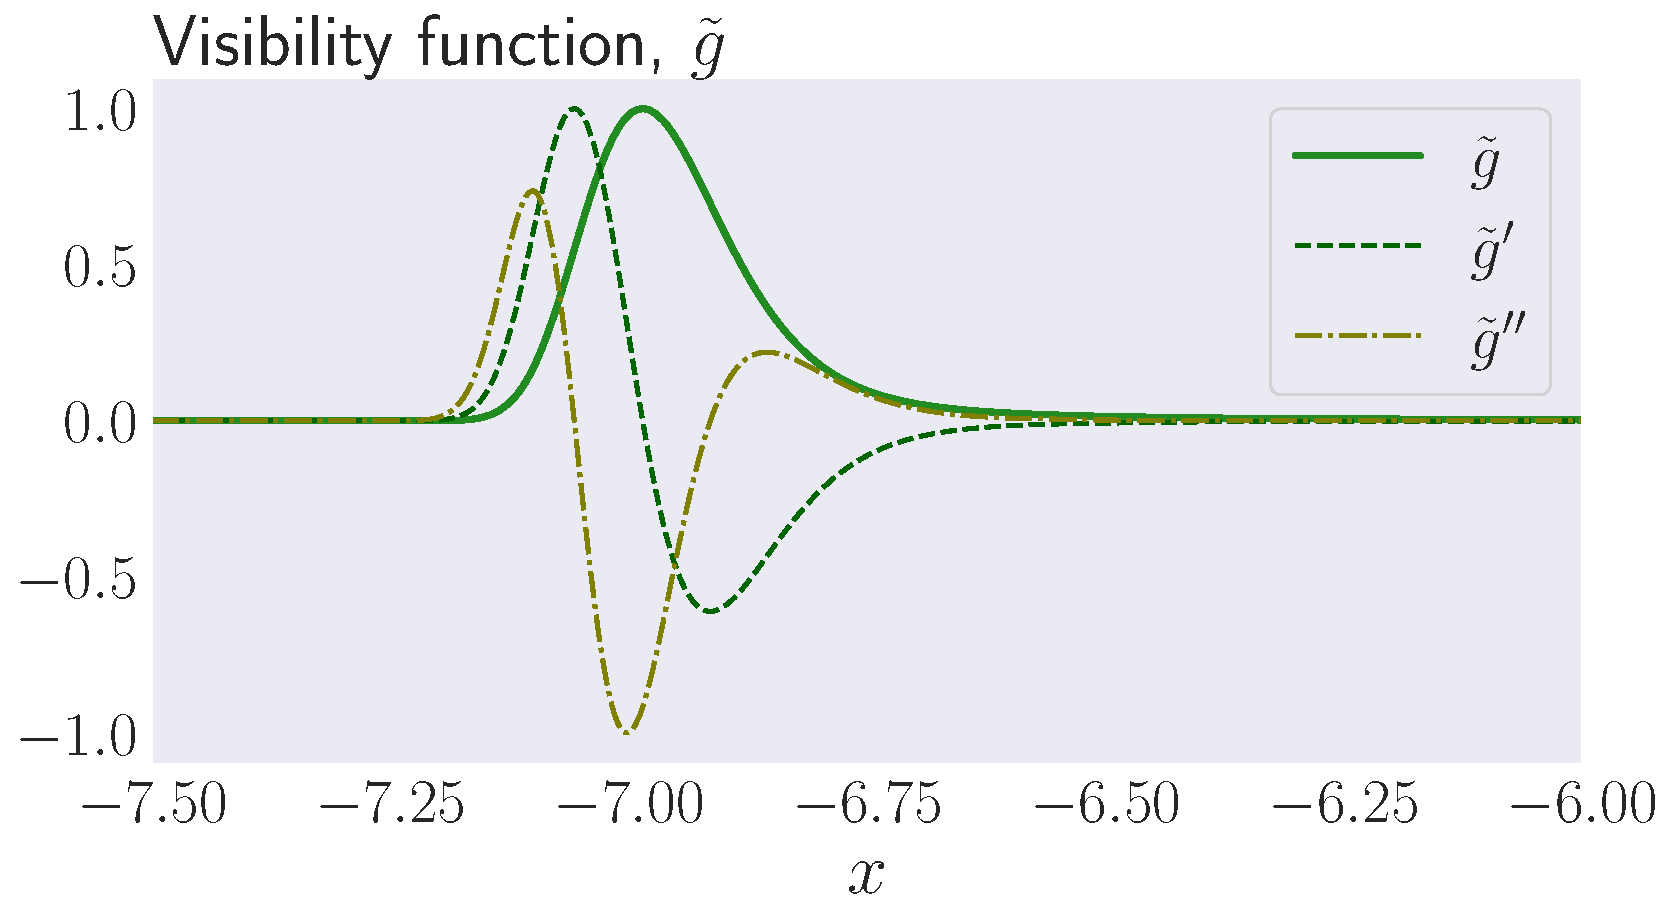
\includegraphics[width=\linewidth]{visibility_function.pdf}
        \caption{The visibility function $\tilde{g}$ and its first and second derivatives as functions of $x$. The time of last scattering is shown as a dashed black line, which by definition coincides with the peak of the visibility function.}
        \label{fig:m2:visibility_function}
    \end{figure}

    \subsubsection{General discussion}
    One key thing to keep in mind is that recombination did not happen instantaneously, but rather over a relatively short period in which neutral hydrogen formed rapidly. This caused a rapid decrease of the free electron fraction, which again caused the optical depth to decrease by several magnitudes. In the same period, we see a that the visibility function is non-zero, meaning the probability of last scattering is (relatively) very high in this period. The times quoted in ~\cref{tab:m2:recomb_analysis} are times that arise from our quite rigid, but fair definition of last scattering and recombination. However, these times do not encapsulate the duration of the abovementioned period.  One could also define the last scattering surface as the time when $\tau=1$ which is the transition between optically thick and optically thin media (when the photon travels exactly one mean free path before scattering). However, the visibility function is arguably a better choice since this is a proper probability distribution, so its peak represents the \textit{actual} time when the probability of last scattering was the highest. Nevertheless, if we change these definitions we ought to expect different times as a result.



